\documentclass[xcolor=table, 8pt]{beamer}

\usetheme[progressbar=foot, sectionpage=none]{metropolis}           % Use metropolis theme

\usepackage{pifont}
\usepackage{booktabs}
\usepackage{appendixnumberbeamer}
\usepackage{colortbl}
\usepackage[font=small,labelfont=bf]{caption}
\usepackage{subcaption}
\usepackage{multirow}
\usepackage[style=authoryear, labelnumber]{biblatex}
\usepackage{xparse}
\usepackage[absolute,overlay]{textpos}
\usepackage{fontawesome5}
\usepackage{algorithm,algorithmic}
\usepackage{nameref}
\usepackage{adjustbox}
\usepackage{tikz}
\usepackage{url}
\usetikzlibrary{positioning}

\makeatletter
\newcommand*{\currentname}{\@currentlabelname}
\makeatother
\usetikzlibrary{calc,shapes.arrows,decorations.pathreplacing, decorations.text}
\addbibresource{bibliography.bib}



\setbeamerfont{caption}{size=\tiny}

\usepackage{totcount}

\newcounter{totalsection}
\regtotcounter{totalsection}

\AtBeginDocument{%
    \pretocmd{\section}{\refstepcounter{totalsection}}{\typeout{Yes, prepending was successful}}{\typeout{No, prepending was not it was successful}}%
}%

\makeatletter
\setbeamertemplate{footline}
{
  \leavevmode%
  \hbox{%
  \begin{beamercolorbox}[wd=.95\paperwidth,ht=2.25ex,dp=1ex,left]{author in head/foot}%
    % \usebeamerfont{author in head/foot} Pierre Le Jeune - 
    \hspace*{1em} \usebeamerfont{title in head/foot}\insertshorttitle\hspace*{3em}
  \end{beamercolorbox}%
  \begin{beamercolorbox}[wd=.05\paperwidth,ht=2.25ex,dp=1ex,right]{title in head/foot}%

    \insertframenumber{} \hspace*{1ex}
  \end{beamercolorbox}}%
  \vskip0pt%
  \setlength{\metropolis@progressinheadfoot@linewidth}{1pt}
  \setlength{\metropolis@titleseparator@linewidth}{1pt}
  \setlength{\metropolis@progressonsectionpage@linewidth}{1pt}
  \typeout{Section}
  \typeout{\thesection}
  \typeout{Tot section}
  \typeout{\totvalue{totalsection}}
  % \typeout{Ratio}
  % \typeout{\ratio{\thesection pt}{\totvalue{totalsection}}
  \setlength{\metropolis@progressonsectionpage}{%
    \textwidth * \ratio{\insertframenumber pt}{\inserttotalframenumber pt}%
  }%
  \begin{beamercolorbox}[wd=\paperwidth]{progress bar in head/foot}
    \begin{tikzpicture}
      \fill[bg] (0,0) rectangle (\textwidth, \metropolis@progressonsectionpage@linewidth);
      \fill[fg] (0,0) rectangle (\metropolis@progressonsectionpage, \metropolis@progressonsectionpage@linewidth);
    \end{tikzpicture}%
  \end{beamercolorbox}

}
\makeatother


% \makeatletter
% \setlength{\metropolis@progressinheadfoot@linewidth}{1pt}
% \setlength{\metropolis@titleseparator@linewidth}{1pt}
% \setlength{\metropolis@progressonsectionpage@linewidth}{1pt}

% \setbeamertemplate{progress bar in section page}{
%   \setlength{\metropolis@progressonsectionpage}{%
%     \textwidth * \ratio{\insertframenumber pt}{\inserttotalframenumber pt}%
%   }%
%   \begin{tikzpicture}
%     \fill[bg] (0,0) rectangle (\textwidth, \metropolis@progressonsectionpage@linewidth);
%     \fill[fg] (0,0) rectangle (\metropolis@progressonsectionpage, \metropolis@progressonsectionpage@linewidth);
%   \end{tikzpicture}%
% }
% \makeatother





\usepackage{tabto}    
\newcommand\sectiontab{\tab \hspace{-5.7cm}}

\newenvironment{sectionframe}[1]
  {
    \begin{frame}{\thesection. \sectiontab #1}
  }
  {
    \end{frame}
  }

  \newenvironment{subsectionframe}[1]
  {
    \begin{frame}{\thesection.\thesubsection \sectiontab #1 - \currentname}
  }
  {
    \end{frame}
  }

  \newenvironment{subsectionframemod}[1]
  {
    \begin{frame}{\thesection.\thesubsection \sectiontab \currentname}
  }
  {
    \end{frame}
  }
\newenvironment{tickenv}
  {\only{%
  \setbeamertemplate{itemize item}{\textbullet}
  \setbeamertemplate{itemize subitem}{\textbullet}
  \setbeamertemplate{itemize subsubitem}{\textbullet}}}
  {}


% Change bibliography font size
\renewcommand*{\bibfont}{\tiny}
% Change bibliography item label size
\renewcommand{\pgfuseimage}[1]{\scalebox{.75}{\includegraphics{#1}}}

% Change bibliography left margin
\defbibenvironment{bibliography}
  {\list{}
     {\settowidth{\labelwidth}{\usebeamertemplate{bibliography item}}%
      \setlength{\leftmargin}{\labelwidth}%
      \setlength{\rightmargin}{\labelwidth}%
      \setlength{\labelsep}{\biblabelsep}%
      \addtolength{\leftmargin}{\labelsep}%
      \setlength{\itemsep}{\bibitemsep}%
      \setlength{\parsep}{\bibparsep}}}
  {\endlist}
  {\item}


% \newcommand{\graphicsbox}[3]{
%   \begin{tikzpicture}
%     \node[anchor=south west,inner sep=0] (image) at (0,0) {\includegraphics[width=0.9\textwidth]{#1}};
%     \begin{scope}[x={(image.south east)},y={(image.north west)}]
%         \draw[red,ultra thick] (0.62,0.65) rectangle (0.78,0.75);
%     \end{scope}
%   \end{tikzpicture}
% }

\newcommand{\nth}[2]{
  \foreach \x [count=\k] in #1 {
        \ifnum\k=#2
            \x
        \fi
    }
}


\NewDocumentCommand{\graphicsbox}{ m m m m O{40mm} O{0.1mm}}{%
  \begin{tikzpicture}
    \node[anchor=south west,inner sep=0] (image) at (0,0) {\includegraphics[width=#5]{#1}};
    
      \begin{scope}[x={(image.south east)},y={(image.north west)}]
        \foreach \pos [count=\k] in {#2}{
          \foreach \size [count=\i] in {#3}{
            \foreach \col [count=\l] in {#4}{
              \ifnum \k = \i
                \ifnum \k = \l
                  \draw[\col , line width=#6] \pos rectangle +\size;
                \fi
            \fi
            }
            
          }
          
        }
      \end{scope}

  \end{tikzpicture}

}

\NewDocumentCommand{\graphicsboxh}{ m m m m O{40mm} O{0.1mm}}{%
  \begin{tikzpicture}
    \node[anchor=south west,inner sep=0] (image) at (0,0) {\includegraphics[height=#5]{#1}};
    
      \begin{scope}[x={(image.south east)},y={(image.north west)}]
        \foreach \pos [count=\k] in {#2}{
          \foreach \size [count=\i] in {#3}{
            \foreach \col [count=\l] in {#4}{
              \ifnum \k = \i
                \ifnum \k = \l
                  \draw[\col , line width=#6] \pos rectangle +\size;
                \fi
            \fi
            }
            
          }
          
        }
      \end{scope}

  \end{tikzpicture}

}


\setbeamertemplate{endpage}{%
    \begin{frame}[plain]
      \centering
      \begin{minipage}{22em}
        % \raggedright
        \centering
        \huge
        \usebeamercolor[fg]{section title}
        \usebeamerfont{section title}
        Thank you for your attention\\[-1ex]
        \usebeamertemplate*{title separator}
        \par
      \end{minipage}
      
    
      \begin{textblock*}{50mm}(39mm,57mm)
        {\large Any questions \faQuestionCircle \\}
      \end{textblock*}

      \begin{textblock*}{100mm}(-18mm,85mm)
        {\faEnvelope \quad hicham.talaoubrid1@edu.univ-paris13.fr \\}
      \end{textblock*}
      
    \end{frame}
}

\newcommand{\bfalert}[1]{\textbf{\alert{#1}}}

\definecolor{l2tiblue}{RGB}{35, 49, 138}
% \title[Representation Learning for FSOD]{Experience feedback using Representation Learning for Few-Shot Object Detection on Aerial Images}
\title[IGARSS 2024 - COSE - L2TI --- Improving Few-Shot and Cross-Domain Object Detection on Aerial Images with a Diffusion-Based Detector.]{Improving Few-Shot and Cross-Domain Object Detection on Aerial Images with a Diffusion-Based Detector.}
\date{}


\author[Short Name (U ABC)]{%
    \texorpdfstring{%
        \begin{columns}[T]
            \column{.33\linewidth}
            \centering
            \textbf{Pierre Le Jeune} \\ \emph{\scriptsize{L2TI, Université Sorbonne Paris Nord \\ \vspace{-1mm}COSE}}
            \column{.33\linewidth}
            \centering
            \textbf{\underline{Hicham Talaoubrid}} \\ \emph{\scriptsize{L2TI, Université Sorbonne Paris Nord \\ \vspace{-1mm}COSE}}
            \column{.33\linewidth}
            \centering
            \textbf{Anissa Mokraoui} \\ \vspace{-1mm}\emph{\scriptsize{L2TI, Université Sorbonne Paris Nord}}
        \end{columns}
        \vspace{5mm}
    }{}
}

% \institute{\vspace{2mm} \normalsize \textbf{Pierre Le Jeune} \\ \small L2TI (UR 3043), Université Sorbonne Paris Nord, COSE}


\titlegraphic{
    \vspace{70mm}
% \scriptsize{\emph{\textsuperscript{1}Université Sorbonne Paris Nord}}

    \begin{textblock}{12}(1.25, 11)
        \textcolor{l2tiblue}{\normalsize{2024 IEEE International Geoscience and Remote Sensing Symposium}} \\
        \small{\emph{July 11, 2024}}
    \end{textblock}

    \begin{tikzpicture}[remember picture,overlay]
        \node[xshift=-2cm,yshift=1.1cm] at (current page.south east){%
            \includegraphics[width=2cm]{Figures/cose_left}};
        \node[xshift=2cm,yshift=1cm] at (current page.south west){%
            \includegraphics[width=1.5cm]{Figures/l2ti}};
        \node[xshift=-1.5cm,yshift=-0.8cm] at (current page.north east){%
            \includegraphics[width=2cm]{./Figures/logo_USPN}};
    \end{tikzpicture}
}



% \renewcommand{\seriesdefault}{ul}

%\setsansfont[BoldFont={Fira Sans Bold},
%    UprightFont={Fira Sans Medium},
%    ItalicFont={Fira Sans MediumItalic}]{Fira Sans Book}
% \setmainfont[BoldFont={Fira Sans SemiBold}]{Fira Sans Book}

\begin{document}
%    \setsansfont[BoldFont={Fira Sans Bold},
%        UprightFont={Fira Sans Medium},
%        ItalicFont={Fira Sans MediumItalic}]{Fira Sans Book}
    \maketitle
%    \setsansfont[BoldFont={Fira Sans SemiBold},
%        UprightFont={Fira Sans Regular},
%        ItalicFont={Fira Sans Italic}]{Fira Sans Book}
    \begin{frame}{Sommaire}
    \setcounter{tocdepth}{1}
    \setbeamertemplate{section in toc}[sections numbered]
    \textbf{\tableofcontents}
    
\end{frame}


%         \item Definition of what is FSOD
%         \item Faster R-CNN, a generic solution for object detection
%         \item Prototypical networks
%         \item Prototypical Faster R-CNN
%         \item Results and analysis
 


    \section{Introduction à la détection d'objet et la détection d'objet few-shot}\label{sec:od-fsod}

    \subsection{Introduction - Principe de la détection d'objet}\label{subsec:object-detection}
    \begin{subsectionframemod}{Object Detection}
    \metroset{block=fill}
    \vspace{-10mm}
    \begin{alertblock}{Principe de la détection d'objets}
        Étant donné un ensemble de classes $\mathcal{C}$, il s'agit de trouver toutes les occurrences d'objets
        appartenant à une classe $c \in \mathcal{C}$ dans une image $I$. Chaque objet est représenté par $(x_1, y_1, x_2, y_2, c)$.
    \end{alertblock}

    \vspace{5mm}
    \pause
    \begin{columns}
        \begin{column}{0.3\textwidth}
            \centering
            \begin{tikzpicture}
                \node[anchor=south west,inner sep=0, label=below:{\small Image d'entrée $I$}] at (0,0){
                    \includegraphics[width=30mm]{Figures/P0770.jpg}
                };
               
            \end{tikzpicture}
            
        \end{column}
        \pause
        
        \begin{column}{0.3\textwidth}
            

            \only<4->{
                \begin{textblock*}{50mm}(41mm,53mm)
                    \huge $\rightarrow$
                \end{textblock*}
                

                \begin{tikzpicture}[remember picture,overlay]
                    \node[xshift=\paperwidth/2 +0mm,yshift=-\paperheight/2- 5mm] at (current page.north west){%
                        \fbox{\parbox[][10mm][c]{0.8\textwidth}{\centering\normalsize Modèle de détection}}
                    };
                \end{tikzpicture}
            }
            % \graphicsbox{Figures/P0131.jpg}{(0.2,0.2)}{(0.23,0.5)}{green}[20mm][0.2mm]
        \end{column}
        \pause
        \begin{column}{0.3\textwidth}
            \only<5->{
                \begin{textblock*}{50mm}(82mm,53mm)
                    \huge $\rightarrow$
                \end{textblock*}
                \centering
                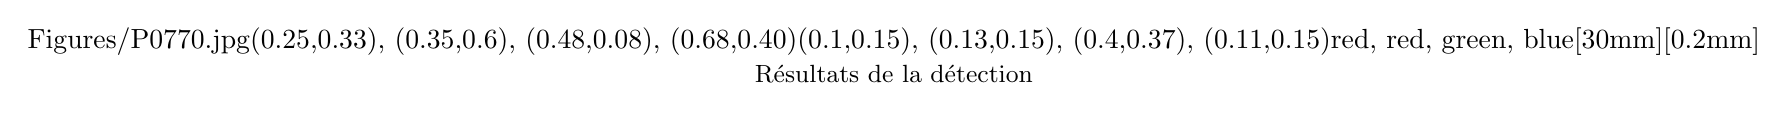
\begin{tikzpicture}
                    \node[anchor=south west,inner sep=0, label=below:{\small Résultats de la détection}] at (0,0){
                        \graphicsbox{Figures/P0770.jpg}{(0.25,0.33), (0.35,0.6), (0.48,0.08), (0.68,0.40)}{(0.1,0.15), (0.13,0.15), (0.4,0.37), (0.11,0.15)}{red, red, green, blue}[30mm][0.2mm]
                    };
                
                \end{tikzpicture}
            }
            
        \end{column}
    \end{columns}
    
    \only<3->{
    \begin{textblock}{12}(2, 12)
        \[ \mathcal{C} = \{ \text{Terrain de baseball, Piscine, Piste d'athlétisme} \}\]
      \end{textblock}
    }
        
\end{subsectionframemod}


    \section{Détection d'objet few-shot}\label{sec:fs-od-fsod}

    \subsection{Introduction - Principe de la détection d'objet few-shot}\label{subsec:fs-od-definition}
    \begin{subsectionframemod}{Few-Shot Object Detection}
    \metroset{block=fill}
    \vspace{-10mm}
    \begin{alertblock}{Détection d'objets $n$-way $k$-shot}
        Étant donné des exemples de support $\{(x_1, a_1), \dots, (x_{nk}, a_{nk})\}$, il s'agit de détecter toutes les occurrences des classes dans $\mathcal{C}$ ($|\mathcal{C}| = n$) dans une image de requête $x_q$.
        En règle générale, $k$ est compris entre 1 et 50.
    \end{alertblock}

    \vspace{5mm}
    \pause
    \begin{columns}
        \begin{column}{0.3\textwidth}
            \centering
            \begin{tikzpicture}
                \node[anchor=south west,inner sep=0, label=below:{\small Query image}] at (0,0){
                    \includegraphics[width=30mm]{Figures/P0770}
                };
               
            \end{tikzpicture}
            
        \end{column}
        \pause
        
        \begin{column}{0.3\textwidth}
            
            \begin{tikzpicture}[remember picture,overlay]
                \only<3->{
                    \node[xshift=\paperwidth/2,yshift=-\paperheight/2-32mm, label=below:{\small $n$ classes, $k$ images par classes}](support) at (current page.north west){%

                    \graphicsbox{Figures/P0131.jpg}{(0.2,0.2)}{(0.23,0.5)}{green}[15mm][0.2mm]
                    \graphicsbox{Figures/P0168.jpg}{(0.26,0.38)}{(0.07,0.07)}{blue}[15mm][0.2mm]
                    \graphicsbox{Figures/P0352.jpg}{(0.6,0.18)}{(0.3,0.3)}{red}[15mm][0.2mm]
                    };
                }
                
                
                \only<4->{\draw[decorate, decoration ={brace,raise=1pt}] (support.north west) -- (support.north east)
                    node (supportlabel) [midway, above=10pt] {\huge $\uparrow$};}

            \end{tikzpicture}
            \only<4->{
                \begin{textblock*}{50mm}(41mm,53mm)
                    \huge $\rightarrow$
                \end{textblock*}
                

                \begin{tikzpicture}[remember picture,overlay]
                    \node[xshift=\paperwidth/2 +0mm,yshift=-\paperheight/2- 5.5mm] at (current page.north west){%
                        \fbox{\parbox[][10mm][c]{0.8\textwidth}{\centering\normalsize Modèle de détection few-shot}}
                    };
                \end{tikzpicture}
            }
            % \graphicsbox{Figures/P0131.jpg}{(0.2,0.2)}{(0.23,0.5)}{green}[20mm][0.2mm]
        \end{column}
        \pause
        \begin{column}{0.3\textwidth}
            \only<5->{
                \begin{textblock*}{50mm}(82mm,53mm)
                    \huge $\rightarrow$
                \end{textblock*}
                \centering
                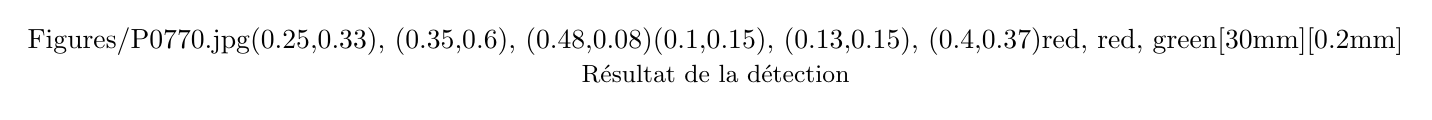
\begin{tikzpicture}
                    \node[anchor=south west,inner sep=0, label=below:{\small Résultat de la détection}] at (0,0){
                        \graphicsbox{Figures/P0770.jpg}{(0.25,0.33), (0.35,0.6), (0.48,0.08)}{(0.1,0.15), (0.13,0.15), (0.4,0.37)}{red, red, green}[30mm][0.2mm]
                    };
                
                \end{tikzpicture}
            }
            
        \end{column}
    \end{columns}
        
\end{subsectionframemod}

    \subsection{Introduction - Challenges de la détection d'objet few-shot sur les images aériennes}\label{sec:fs-od-challenges}
    \begin{subsectionframemod}{Difference between Natural and Aerial Images}
    La plupart des méthodes sont évaluées sur des images naturelles : les ensembles de données Pascal VOC et MS COCO.
    $\Rightarrow$ cela ne garantit pas de bonnes performances sur les images aériennes.
    \vspace{2mm}


    Les tailles des objets sont extrêmement différentes entre les images aériennes et naturelles.

    \begin{figure}
        \includegraphics[width=0.8\textwidth]{Figures/object_sizes.png}
    \caption{Diagramme en boîte des tailles d'objets dans DOTA (\cite{xia2018dota}), DIOR (\cite{li2020object}) et Pascal VOC (\cite{everingham2010pascal}); par classe \textbf{(à droite)} et globalement \textbf{(à gauche)}.}
    \end{figure}

    

    
\end{subsectionframemod}
%    \input{Frames/frame_smoanalysis}

    \section{Axes de recherche autour de la détection d'objet few-shot cross-domain}\label{subsec:fs-od-cd}
    \subsection{Principe de la détection d'objet few-shot cross-domain}\label{subsec:fs-od-cd-principle}
    \begin{subsectionframemod}{Cross-Domain Few-Shot Object Detection}
    \metroset{block=fill}
    \vspace{-10mm}
    \begin{alertblock}{Détection d'objet few-shot cross-domain}
        Dans la détection d'objets à faible échantillon inter-domaines (CD-FSOD), deux ensembles de données distincts sont utilisés pendant l'entraînement de base et l'affinage.
        La CD-FSOD est plus difficile, car le modèle doit non seulement s'adapter à de nouvelles classes, mais aussi à de nouvelles images.
    \end{alertblock}
    \vspace{5mm}

    \only<1>{
        \begin{figure}
            \centering
            \includegraphics[width=0.6\textwidth]{Figures/cross_domain_1}
        \end{figure}
    }
    \pause
    \only<2>{
        \begin{figure}
            \centering
            \includegraphics[width=0.6\textwidth]{Figures/cross_domain_2}
        \end{figure}
    }
    \pause
    \only<3>{
        \begin{figure}
            \centering
            \includegraphics[width=0.6\textwidth]{Figures/cross_domain_3}
        \end{figure}
    }
    \pause
    \only<4>{
        \begin{figure}
            \centering
            \includegraphics[width=0.6\textwidth]{Figures/cross_domain_4}
        \end{figure}
    }

\end{subsectionframemod}
    \subsection{3 Axes de recherche principaux}\label{subsec:fs-od-cd-research}
    \begin{subsectionframemod}{Publications}
    \textbf{Les principaux travaux réalisés au cours de l'année :}
    \textbf{Principaux travaux réalisés au cours de l'année :}
    \begin{itemize}
        \item[-] Développement d'un outil permettant de comparer rapidement et efficacement les performances des modèles d'intelligence artificielle les plus performants.
        \item[-] Mise en évidence de l'importance du choix d'un dataset source pertinent, avec une estimation de l'écart inter-domaines pour identifier le dataset source le plus adapté.
        \item[-] Limitation du risque d'overfitting afin d'assurer une meilleure généralisation des modèles et, par conséquent, d'améliorer leurs performances.
    \end{itemize}

\end{subsectionframemod}


    \subsection{Etat de l'art des modèles de cross-domain}\label{subsec:fs-od-cd-sota}
    \begin{subsectionframemod}{Détection d'objet few-shot}

    \vspace{-3mm}
    \begin{table}[h]

    \label{tab:comparison}
    \begin{adjustbox}{width=0.75\textwidth}
        \rowcolors{2}{gray!25}{white}
        % \begin{tabular}{lllTLLT}
        \begin{tabular}{@{}llccc}
            \toprule[1pt]
            \textbf{Approach}                                                                    & \textbf{Name}                                      & \textbf{Framework}         & \textbf{Episodic Training}  & \textbf{Datasets}                  \\ \hline
            \cellcolor{white}                                                                    &  FRW \parencite{kang2019few}                        & YOLO (no FPN)              & Yes                         & Pascal / COCO                     \\
            \cellcolor{white}                                                                    & RSI   \parencite{deng2020few}                     & YOLO                       & Yes                         & DIOR / NWPU VHR                    \\
            \cellcolor{white}                                                                    & MRCNN \parencite{yan2019meta}                     & Faster R-CNN (no FPN)      & Yes                         & Pascal / COCO                      \\
            \cellcolor{white}                                                                    & ARMRD \parencite{fan2020fsod}                     & Faster R-CNN               & No                          & COCO                               \\
            \cellcolor{white}                                                                    & VEOW  \parencite{xiao2020few}                     & Faster R-CNN               & No                          & Pascal / COCO                      \\
            \cellcolor{white}                                                                    & SAA \parencite{xiao2020fsod}                    & Faster R-CNN               & No                          & RSOD / NWPU VHR                    \\
            \cellcolor{white}                                                                    & CACE  \parencite{wallach2019one}                  & Faster R-CNN               & No                          & Pascal / COCO                      \\
            \cellcolor{white}                                                                    & KT    \parencite{kim2020few}                      & Faster R-CNN               & No                          & Pascal                             \\
            \cellcolor{white}                                                                    & IFSOD \parencite{ganea2021incremental}            & Center Ne (no FPN)         & Yes                         & Pascal / COCO / Deepfashion        \\
            \cellcolor{white}                                                                    & WOFT  \parencite{li2020one}                       & FCOS                       & Yes                         & Pascal / COCO                      \\
            \cellcolor{white}                                                                    & FPDI  \parencite{gao2021fast}                     & Faster R-CNN               & No                          & DOTA /  NWPU VHR                   \\
            \cellcolor{white}                                                                    & MFRCN \parencite{han2021meta}                     & Faster R-CNN               & No                          & Pascal / COCO                      \\
            \cellcolor{white}                                                                    & MDETR \parencite{zhang2021meta}                   & DETR (no FPN)              & No                          & Pascal / COCO                      \\
            \cellcolor{white}                                                                    & DRL   \parencite{liu2021dynamic}                  & Faster R-CNN               & Yes                         & Pascal / COCO                      \\
            \cellcolor{white}                                                                    & DANA  \parencite{chen2021should}                  & Faster R-CNN and RetinaNet & Yes                         & Pascal / COCO                      \\
            \cellcolor{white}                                                                    & SP    \parencite{xu2021few}                       & Faster R-CNN               & No                          & Pascal / COCO                      \\
            \cellcolor{white}                                                                    & JCACR \parencite{chu2021joint}                    & YOLO                       & No                          & Pascal / COCO                      \\
            \cellcolor{white}                                                                    & TI \parencite{li2021transformation}               & Faster R-CNN               & Yes                         & Pascal / COCO                      \\
            \multirow{-19}{*}[0mm]{\cellcolor{white}\textbf{Attention}}                          & FCT \parencite{han2022few}                        & Faster R-CNN               & No                          & Pascal / COCO                      \\ \hline
            \cellcolor{white}                                                                    & PNPDet\parencite{zhang2021pnpdet}                 & Center Net (no FPN)        & No                          & Pascal / COCO                      \\
            \cellcolor{white}                                                                    & UPE   \parencite{wu2021universal}                 & Faster R-CNN               & No                          & Pascal / COCO                      \\
            \multirow{-3}{*}[0mm]{\cellcolor{white}\parbox{1.5cm}{\textbf{Attention/ Metric}}}   & GD \parencite{liu2021gendet}                      & FCOS                       & Yes                         & Pascal / COCO                      \\ \hline
            \cellcolor{white}                                                                    & RM    \parencite{karlinsky2019repmet}             & Faster R-CNN               & No                          & Pascal / ImageNet Loc              \\
            \cellcolor{white}                                                                    & RNI \parencite{yang2020restoring}                 & Faster R-CNN               & No                          & Pascal / ImageNet Loc              \\
            \cellcolor{white}                                                                    & FSCE  \parencite{sun2021fsce}                     & Faster R-CNN               & No                          & Pascal / COCO                      \\
            \cellcolor{white}                                                                    & PFRCN \parencite{jeune2021experience}             & Faster R-CNN               & Yes                         & DOTA / DIOR                        \\
            \cellcolor{white}                                                                    & AD \parencite{cao2021few}                         & Faster R-CNN               & No                          & Pascal / COCO                      \\
            \multirow{-6}{*}{\cellcolor{white}\parbox{1.5cm}{\textbf{Metric Learning}}}          & GDSVD \parencite{wu2021generalized}               & Faster R-CNN               & No                          & Pascal / COCO                      \\ \hline
            \cellcolor{white}                                                                    & LSTD  \parencite{chen2018lstd}                    & Faster R-CNN               & No                          & Pascal / COCO                      \\
            \cellcolor{white}                                                                    & WOFG  \parencite{fan2021generalized}              & Faster R-CNN               & No                          & Pascal / COCO                      \\
            \cellcolor{white}                                                                    & TFA   \parencite{wang2020frustratingly}           & Faster R-CNN               & No                          & Pascal / COCO                      \\
            \cellcolor{white}                                                                    & MSPSR \parencite{wu2020multi}                     & Faster R-CNN               & No                          & Pascal / COCO                      \\
            \cellcolor{white}                                                                    & DETRG \parencite{bar2022detreg}                   & Faster R-CNN               & No                          & COCO                               \\
            \cellcolor{white}                                                                    & HFSOD \parencite{zhang2021hallucination}          & Faster R-CNN               & No                          & Pascal / COCO                      \\
            \cellcolor{white}                                                                    & DHP \parencite{wolf2021double}                    & Faster R-CNN               & No                          & iSAID /  NWPU VHR                  \\
            \cellcolor{white}                                                                    & SAM \parencite{huang2021few}                      & Faster R-CNN               & No                          & DIOR / NWPU VHR                    \\
            \multirow{-9}{*}{\cellcolor{white}\parbox{1.5cm}{\textbf{Fine-tuning}}}              & SIMPL \parencite{xu2022simpl}                     & Faster R-CNN (no FPN)      & No                          & xView (plane only)                 \\ \bottomrule[1pt]
            \end{tabular}%
    \end{adjustbox}
    \caption{Comparison of the FSOD methods from an attention perspective. All
    frameworks are working with multiscale features except for the one with the
    mention no FPN.}

\end{table}
\end{subsectionframemod}

\begin{subsectionframemod}{Détection d'objet few-shot}

    \vspace{-3mm}
    \begin{table}[h]

    \label{tab:comparison}
    \begin{adjustbox}{width=0.75\textwidth}
        \rowcolors{2}{gray!25}{white}
        % \begin{tabular}{lllTLLT}
        \begin{tabular}{@{}lc}
            \begin{tabular}{@{}lcc}
                \toprule[1pt]
                & \textbf{DOTA} & \textbf{DIOR} \\ \hline
                Few-shot              & 60.45         & 57.51         \\
                Cross-domain Few-shot (COCO) & 25.02         & 38.73         \\\bottomrule[1pt]
                Cross-domain Few-shot (DOTA) & \_         & 38.44         \\\bottomrule[1pt]
                Cross-domain Few-shot (DIOR) & 33.30         & \_         \\\bottomrule[1pt]
            \end{tabular}%
        \end{tabular}%
    \end{adjustbox}
    \caption{Comparaison des performances de DiffusionDet (\cite{chen2022diffusiondet}) en Few-shot et en Cross-domain Few-shot sur DOTA et DIOR en considérant 3 dataset source (notés entre paranthèse) avec 10 shots.}

\end{table}
\end{subsectionframemod}


    \subsection{Importance du dataset source}\label{subsec:srcdata}
    \begin{subsectionframemod}{Détection d'objet few-shot}

    \begin{table}[]
    \centering
    \resizebox{0.9\columnwidth}{!}{%
        \begin{tabular}{@{\hspace{2mm}}cccccccccc@{\hspace{2mm}}}
            \toprule
            \textbf{$k$ shots} & \textbf{DOTA $\to$ DIOR} & & \textbf{COCO $\to$ DIOR} & & \textbf{DIOR $\to$ DOTA} & & \textbf{COCO $\to$ DOTA}      \\ \midrule
            \textbf{1}         & \textbf{20.18}           & & 11.10                    & & \textbf{5.41}            & & 4.03                     \\
            \textbf{5}         & \textbf{34.43}           & & 30.42                    & & \textbf{25.88}           & & 14.45                    \\
            \textbf{10}        & \textbf{41.48}           & & 38.73                    & & \textbf{31.99}           & & 25.02                    \\
            \textbf{20}        & \textbf{49}              & & 48.23                    & & \textbf{38.77}           & & 33.31                    \\
            \textbf{50}        & 54.07                    & & \textbf{56.97}                    & & \textbf{44.07}           & & 43.23                    \\ \bottomrule[1pt]
        \end{tabular}%
    } \caption{Comparaison des performances de FSDiffusionDet en utilisant différents datasets sources pour la détection d'objet cross-domain.
    Les performances sont évaluées en mAP (\%) rapporté avec un seuil IoU à 0.5.}
    \label{tab:cd_fsod_dota2dior}
    \vspace{-1.5em}
\end{table}
\end{subsectionframemod}



    \subsection{Estimation de l'écart entre domaines}\label{subsec:results-variances}
    \begin{subsectionframemod}{Cross-Domain Few-Shot Object Detection}

    \only<1>{
        \begin{figure}
            \centering
            \includegraphics[width=\textwidth]{Figures/cross_domain_1}
            \caption{Schema de la méthode utilisé pour tenter d'estimer le domaine shift}
        \end{figure}
    }
    \pause
    \only<2>{
        \begin{figure}
            \centering
            \includegraphics[width=\textwidth]{Figures/embeddings}
            \caption{Schema de la méthode utilisé pour tenter d'estimer le domaine shift}
        \end{figure}
    }
    \pause
    \only<3>{
        \begin{figure}
            \centering
            \includegraphics[width=\textwidth]{Figures/embeddings_pca}
            \caption{Schema de la méthode utilisé pour tenter d'estimer le domaine shift}
        \end{figure}
    }

\end{subsectionframemod}
    \begin{subsectionframemod}{Conclusion}
    \begin{figure}[!t]
        \centering
        \includegraphics[width=0.6\textwidth]{Figures/2d_class_plot.png}
        \caption{Représentation 2D des projections des barycentres de chaque classe, obtenue après le passage des images de chaque dataset dans un modèle pré-entraîné sur COCO, suivi d'une réduction dimensionnelle par PCA.}
        \label{fig:2dclass}
    \end{figure}
\end{subsectionframemod}



    \begin{subsectionframemod}{Difference between Natural and Aerial Images}
    \begin{figure}[!h]
    \centering
    \begin{tabular}{cc}
        \includegraphics[scale=0.25]{Figures/con_sep.png} &
        \includegraphics[scale=0.25]{Figures/ncon_sep.png} \\
        (a) Variance intra-classe faible, & (b) Variance intra-classe forte,\\
         Variance inter-classe forte, & Variance inter-classe forte, \\
         \\
        \includegraphics[scale=0.25]{Figures/con_nsep.png} &
        \includegraphics[scale=0.25]{Figures/ncon_nsep.png}\\
        (d) Variance intra-classe faible, & (c) Variance intra-classe forte, \\
        Variance inter-classe faible,  & Variance inter-classe faible, \\
    \end{tabular}
    \caption{Illustration conceptuelle de la séparabilité des classes en relation avec les variances inter-classes et intra-classes. Les projections dans l'espace latent des images d'une classe sont représentées par des points bleus, tandis que les projections d'une autre classe sont marquées en rouge, avec les barycentres de chaque classe indiqués par des points plus foncés.}
    \label{fig:sep_classes}
\end{figure}
\end{subsectionframemod}




    \begin{subsectionframemod}{Conclusion}
\begin{figure}[!t]
    \centering
    \begin{subfigure}[b]{0.49\textwidth}
         \centering
         \includegraphics[width=\textwidth]{Figures/deepfruits.png}
         \caption{Représentation 2D de la projection des objets de DeepFruits après un PCA avec les barycentres mis en valeur avec des cercles de couleurs.}
         \label{fig:deepfruits}
    \end{subfigure}
    \hfill
    \begin{subfigure}[b]{0.49\textwidth}
         \centering
         \includegraphics[width=\textwidth]{Figures/2d_class_plot.png}
         \caption{Représentation 2D des projections des barycentres de chaque classe de chaque datasets après un PCA.}
         \label{fig:2dclass}
    \end{subfigure}
    \caption{Représentation 2D des projections  (a) des objets du dataset DeepFruits et (b) des barycentres de chaque classe après un PCA.}
    \label{fig:class-representation}
\end{figure}
\end{subsectionframemod}




    \subsection{Méthodes PEFT (Parameter Efficient Fine-Tuning) pour limiter l'overfitting}\label{sec:peft}
    \begin{subsectionframemod}{Difference between Natural and Aerial Images}

    \only<1>{
        \begin{figure}
            \centering
            \includegraphics[width=0.6\textwidth]{Figures/lora_1}
            \caption{Schéma présentant LoRA (Low-Rank Adaptation), une technique permettant entre autre de limiter le risque d'overfitting pour assurer de meilleurs performances.}
        \end{figure}
    }
    \pause
    \only<2>{
        \begin{figure}
            \centering
            \includegraphics[width=0.6\textwidth]{Figures/lora_2}
            \caption{Schéma présentant LoRA (Low-Rank Adaptation), une technique permettant entre autre de limiter le risque d'overfitting pour assurer de meilleurs performances.}
        \end{figure}
    }
    \pause
    \only<3>{
        \begin{figure}
            \centering
            \includegraphics[width=0.6\textwidth]{Figures/lora_3}
            \caption{Schéma présentant LoRA (Low-Rank Adaptation), une technique permettant entre autre de limiter le risque d'overfitting pour assurer de meilleurs performances.}
        \end{figure}
    }
    \pause
    \only<4>{
        \begin{figure}
            \centering
            \includegraphics[width=0.6\textwidth]{Figures/lora_4}
            \caption{Schéma présentant LoRA (Low-Rank Adaptation), une technique permettant entre autre de limiter le risque d'overfitting pour assurer de meilleurs performances.}
        \end{figure}
    }
    \pause
    \only<5>{
        \begin{figure}
            \centering
            \includegraphics[width=0.6\textwidth]{Figures/lora_5}
            \caption{Schéma présentant LoRA (Low-Rank Adaptation), une technique permettant entre autre de limiter le risque d'overfitting pour assurer de meilleurs performances.}
        \end{figure}
    }
    \pause
    \only<6>{
        \begin{figure}
            \centering
            \includegraphics[width=0.6\textwidth]{Figures/lora_5-5}
            \caption{Schéma présentant LoRA (Low-Rank Adaptation), une technique permettant entre autre de limiter le risque d'overfitting pour assurer de meilleurs performances.}
        \end{figure}
    }
    \pause
    \only<7>{
        \begin{figure}
            \centering
            \includegraphics[width=0.6\textwidth]{Figures/lora_6}
            \caption{Schéma présentant LoRA (Low-Rank Adaptation), une technique permettant entre autre de limiter le risque d'overfitting pour assurer de meilleurs performances.}
        \end{figure}
    }


\end{subsectionframemod}
    \begin{subsectionframemod}{Difference between Natural and Aerial Images}

    \begin{figure}
        \includegraphics[width=0.4\textwidth]{Figures/svf.png}
        \caption{SVF (\cite{sun2022singular}) se base sur une décomposition en valeurs singulières. Dans ce cas on entraîne seulement les valeurs singulières.}
    \end{figure}


\end{subsectionframemod}

    \subsection{Premiers résultats avec LoRA}\label{subsec:results-loracurves}
    \begin{subsectionframemod}{Performance Analysis}

\begin{figure}[h]
        \centering
        \begin{subfigure}{0.5\textwidth}
            \includegraphics[width=\textwidth]{Figures/lora4.png}
        \end{subfigure}
        \begin{subfigure}{0.5\textwidth}
            \includegraphics[width=\textwidth]{Figures/lora5.png}
        \end{subfigure}
        \caption{Impact de LoRA sur l'entraînement de FSDiffusionDet sur DIOR en utilisant 10 shots et un rang de 16.}
        \label{fig:lora_curves}
    \end{figure}
\end{subsectionframemod}

\begin{subsectionframemod}{Performance Analysis}

\begin{figure}[h]
        \centering
        \begin{subfigure}{0.45\textwidth}
            \includegraphics[width=\textwidth]{Figures/lora_rank1.png}
        \end{subfigure}
        \begin{subfigure}{0.45\textwidth}
            \includegraphics[width=\textwidth]{Figures/lora_rank2.png}
        \end{subfigure}
        \begin{subfigure}{0.45\textwidth}
            \includegraphics[width=\textwidth]{Figures/lora_rank3.png}
        \end{subfigure}
        \begin{subfigure}{0.45\textwidth}
            \includegraphics[width=\textwidth]{Figures/lora_rank4.png}
        \end{subfigure}
        \caption{Impact du rang de LoRA sur l'entraînement de FSDiffusionDet sur DIOR en utilisant 10 shots.}
        \label{fig:lora_curves2}
    \end{figure}
\end{subsectionframemod}




    \section{Contributions scientifiques}\label{subsec:approach-publications}
    \begin{subsectionframemod}{Publications}
    \textbf{Articles de conférence acceptés (avant la thèse)} :
    \begin{itemize}
        \item[-] Improving Few-Shot and Cross-Domain Object Detection on Aerial Images with a Diffusion-Based Detector --
        accepté et présenté à \bfalert{IGARSS} (7 Juil. 2024) (relecture du papier, participation aux expériences et présentation oral)
    \end{itemize}

    \textbf{Articles de conférence soumis}
    \begin{itemize}
        \item[-] Indirect Attention: IA-DETR for one shot Object Detection -- soumis à \bfalert{ICLR} (2024) (participation au code et aux expériences)
    \end{itemize}

\end{subsectionframemod}



    \section{Travaux future}\label{subsec:approach-future-work}
    \begin{subsectionframemod}{Conclusion}
\begin{itemize}
    \item[-]  Expérimentation pour aider au choix du domaine source en cross domain\\\hfill\bfalert{\tiny{objectif octobre 2024}}
    \item[-]  Travail sur un framework facilitant l'expérimentation en cross domain\\\hfill\bfalert{\tiny{objectif octobre 2024}}
    \item[-]  Utiliser le framework pour réaliser un article benchmark des méthodes cross domain\\\hfill\bfalert{\tiny{objectif novembre 2024}}
    \item[-]  Travaux sur des PEFT qui pourrait fonctionner pour la regression\\\hfill\bfalert{\tiny{objectif début 2025}}
    \item[-]  Compléter le papier du benchmark pour l'inclure dans un journal\\\hfill\bfalert{\tiny{objectif début 2025}}
    \item[-]  Travaux sur les VLM (Vision/Language Models)\\\hfill\bfalert{\tiny{objectif courant 2025}}
\end{itemize}


\end{subsectionframemod}

    \section{Formations}\label{subsec:formations}
    \begin{subsectionframemod}{Publications}
    \textbf{Formation dotorale suivie} :
    \begin{itemize}
        \item[-] Formations professionnalisantes et langues -- Anglais de communication niveau faux débutant-intermédiaire  \bfalert{4 ECTS}
    \end{itemize}

    \textbf{Conférences présentées} :
    \begin{itemize}
        \item[-] Présentation orale à \bfalert{IGARSS} (8-12 Juil.) -- \textit{Improving Few-Shot and Cross-Domain Object Detection on Aerial Images with a Diffusion-Based Detector} \bfalert{24 ECTS}
    \end{itemize}

    \textbf{Mobilité} :
    \begin{itemize}
        \item[-] Mobilité de 4 mois à l'ETS Montréal (Canada)
    \end{itemize}

\end{subsectionframemod}



    \usebeamertemplate{endpage}

    \begin{frame}[allowframebreaks=]{References}
        \printbibliography
    \end{frame}
\end{document}
